\documentclass[conference]{IEEEtran}
\IEEEoverridecommandlockouts
% The preceding line is only needed to identify funding in the first footnote. If that is unneeded, please comment it out.
\usepackage{cite}
\usepackage{amsmath,amssymb,amsfonts}
\usepackage{algorithmic}
\usepackage{graphicx}
\usepackage{textcomp}
\usepackage{hyperref}
\usepackage{xcolor}
\usepackage[section]{placeins}
\def\BibTeX{{\rm B\kern-.05em{\sc i\kern-.025em b}\kern-.08em
    T\kern-.1667em\lower.7ex\hbox{E}\kern-.125emX}}
\begin{document}

\title{
{ 5G Latency Comparison with 4G
}
}

\author{\IEEEauthorblockN{Megha Prajapati}
\IEEEauthorblockA{\textit{202151091} \\
}
\and
\IEEEauthorblockN{Vasireddy Satvika }
\IEEEauthorblockA{\textit{202151175} \\
}
\and
\IEEEauthorblockN{Sanya}
\IEEEauthorblockA{\textit{202152338} \\
}
}

\maketitle
\href{https://github.com/IIITV-5G-and-Edge-Computing-Activity/5G-Latency-Comparison-with-4G}{Access all project-related files here.}
\section{Abstract}
The aim of this project is to evaluate and compare the latency performance of 5G and 4G networks to assess the advancements in response times provided by 5G technology. Focusing on metrics such as round-trip time (RTT), upload latency, and download latency, the study analyzes performance across diverse use cases like gaming, video streaming, and video calls under varying conditions of signal strength and network load. Real-world data collected from devices supporting both networks is analyzed statistically to identify improvements and limitations. The findings provide insights into 5G’s role in enhancing user experiences and supporting latency-critical applications.
\section*{Objective}
The primary objective of this project is to evaluate and compare the latency performance of 5G and 4G networks in real-world scenarios. This involves:

\begin{enumerate}
    \item Measuring key latency metrics, including:
    \begin{itemize}
        \item Round-trip time (RTT)
        \item Upload latency
        \item Download latency
    \end{itemize}
    \item Testing across various use cases, such as:
    \begin{itemize}
        \item Video streaming
        \item Gaming
        \item Video calls
    \end{itemize}
    \item Varying conditions to ensure comprehensive analysis:
    \begin{itemize}
        \item Signal strength
        \item Network load
        \item Geographical locations
        \item Times of day
    \end{itemize}
    \item Collecting data using devices capable of both 4G and 5G networks.
    \item Employing statistical methods to compare 4G and 5G latency data and identify performance improvements.
    \item Visualizing results through graphs and tables to provide clear insights.
\end{enumerate}

The results aim to highlight the advantages and limitations of 5G in terms of latency, providing valuable insights into its effectiveness for latency-sensitive applications.

\section{Introduction}
The evolution of mobile communication networks has been pivotal in shaping modern technology and user experiences. The fifth-generation (5G) network represents a significant leap forward in terms of speed, capacity, and latency compared to its predecessor, the fourth-generation (4G) network. This project focuses on assessing one of the critical aspects of network performance—latency—across 4G and 5G networks.

Latency, defined as the time taken for a data packet to travel from the source to the destination and back (round-trip time), plays a crucial role in determining the responsiveness of applications. From video calls to online gaming and video streaming, low latency is essential for ensuring seamless and real-time user experiences. As 5G aims to support emerging latency-critical applications, such as autonomous vehicles and remote surgeries, understanding its latency performance is vital.

This study explores latency metrics such as round-trip time (RTT), upload latency, and download latency by testing various use cases, including gaming, video streaming, and video calls. Real-world data is collected using devices capable of operating on both 4G and 5G networks. To ensure comprehensive analysis, tests are conducted under varying conditions, including differences in signal strength, network load, geographical locations, and times of day.

Through statistical analysis and visualization, the project highlights the advancements offered by 5G in latency performance, identifies limitations, and provides insights into its potential for enhancing user experiences. The findings aim to shed light on the transformative capabilities of 5G and its effectiveness in meeting the demands of latency-sensitive applications.

\section{Methodology}
This study follows a systematic approach to evaluate and compare the latency performance of 4G and 5G networks across multiple real-world use cases. The methodology is outlined as follows:

\subsection*{Data Collection}
Latency data was collected using Wireshark, a powerful packet analysis tool, on a smartphone capable of supporting both 4G and 5G networks. The study included five distinct use cases to ensure comprehensive evaluation:
\begin{enumerate}
    \item \textbf{Idle State:} The phone was left idle with no active applications to observe baseline network activity and idle state latency.
    \item \textbf{Video Streaming:} A movie was streamed using Prime Video to measure latency during high-bandwidth video playback.
    \item \textbf{Video Call:} A WhatsApp video call was conducted, utilizing features like background filters and effects to simulate typical user interactions.
    \item \textbf{Gaming:} The game \textit{Scott Busters} was played to analyze latency performance during interactive gaming sessions.
    \item \textbf{Downloading:} A series was downloaded using Prime Video to measure latency under heavy download activity.
\end{enumerate}

For each use case, packet capture files (\texttt{.pcap}) were generated for both 4G and 5G networks. The captured data includes detailed information on round-trip time (RTT), upload latency, and download latency. 

\subsection*{Data Analysis}
The captured \texttt{.pcap} files were analyzed to extract relevant latency metrics:
\begin{itemize}
    \item Round-trip time (RTT)
    \item Upload latency
    \item Download latency
\end{itemize}
Wireshark's built-in tools and filters were used to isolate packets relevant to each use case, and the latency values were exported as CSV files for further processing.

\subsection*{Visualization and Statistical Analysis}
The extracted data was processed to generate visualizations that compare latency performance between 4G and 5G networks:
\begin{itemize}
    \item Line graphs illustrating latency trends over time for each use case.
    \item Bar charts comparing average latency across the use cases.
    \item Box plots showcasing the distribution and variability of latency for 4G and 5G.
\end{itemize}

Statistical methods were employed to compute:
\begin{itemize}
    \item Mean, median, and standard deviation for each metric and use case.
    \item Comparative percentage improvements in latency between 4G and 5G.
\end{itemize}

\subsection*{Validation and Enhancements}
To ensure the reliability of the findings:
\begin{itemize}
    \item Multiple tests were conducted for each use case to account for variations in network conditions.
    \item Additional scenarios, such as varying signal strength and testing during different times of the day, were included to analyze the impact of external factors.
\end{itemize}

\section{Wireshark Analysis and Observations}

To understand the network behavior and collect real-world latency data, Wireshark, a powerful network protocol analyzer, was utilized. Screenshots of the packet captures provide insights into the network activity for various use cases and highlight key metrics such as round-trip time (RTT), upload latency, and download latency.

Wireshark captures were conducted for both 4G and 5G networks, ensuring a comprehensive comparison of their latency performance. The packet capture files (\texttt{.pcap}) generated during the experiments were analyzed to extract detailed metrics and trends. Below are some notable screenshots illustrating different aspects of the analysis:

\begin{itemize}
    \item \textbf{Packet Details and Round-Trip Time (RTT):} Screenshots showing the time taken for data packets to travel between the device and the server for each use case.
    \item \textbf{Latency Trends:} Wireshark graphs displaying latency trends over the duration of the activity, providing a real-time view of network responsiveness.
    \item \textbf{Comparison of Upload and Download Latency:} Visual representations of upload and download performance for 4G and 5G networks.
    \item \textbf{Filters and Metrics:} Screenshots demonstrating the use of Wireshark filters to isolate specific packets for analysis, such as \texttt{tcp.analysis.ack\_rtt}.
\end{itemize}

These screenshots not only validate the data collection process but also provide a visual representation of the differences in performance between 4G and 5G networks. Observations from these analyses form the basis for the subsequent statistical and graphical comparisons presented in this report.
\subsection*{5G Network}
The following observations summarize the latency metrics for 5G under different scenarios.
\begin{itemize}
    \item \textbf{Idle (No Activity):}
    \begin{itemize}
        \item \textbf{Time Started:} 32.711532s
        \item \textbf{Minimum Latency:} 27ms
        \item \textbf{Maximum Latency:} 80ms
        \item \textbf{Average Latency:} 52ms
        \item \textbf{Time Ended:} 121.6284s
    \end{itemize}
    \begin{figure}[h]
        \centering
        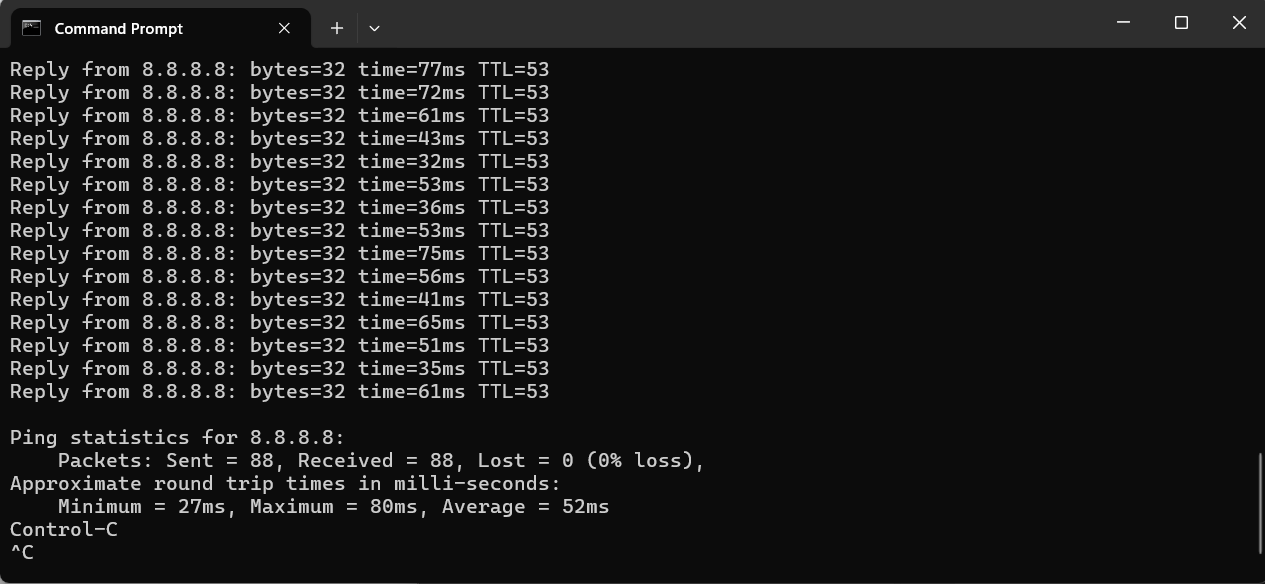
\includegraphics[width=0.8\linewidth]{Image/5g-idle.png}
        \caption{Screenshot for 5G Network Without Activity}
        \label{fig:5g_idle}
    \end{figure}
\newpage
    \item \textbf{Video Streaming:}
    \begin{itemize}
        \item \textbf{Time Started:} 220.8459s
        \item \textbf{Minimum Latency:} 23ms
        \item \textbf{Maximum Latency:} 155ms
        \item \textbf{Average Latency:} 60ms
        \item \textbf{Time Ended:} 340.4930s
    \end{itemize}
    \begin{figure}[h]
        \centering
        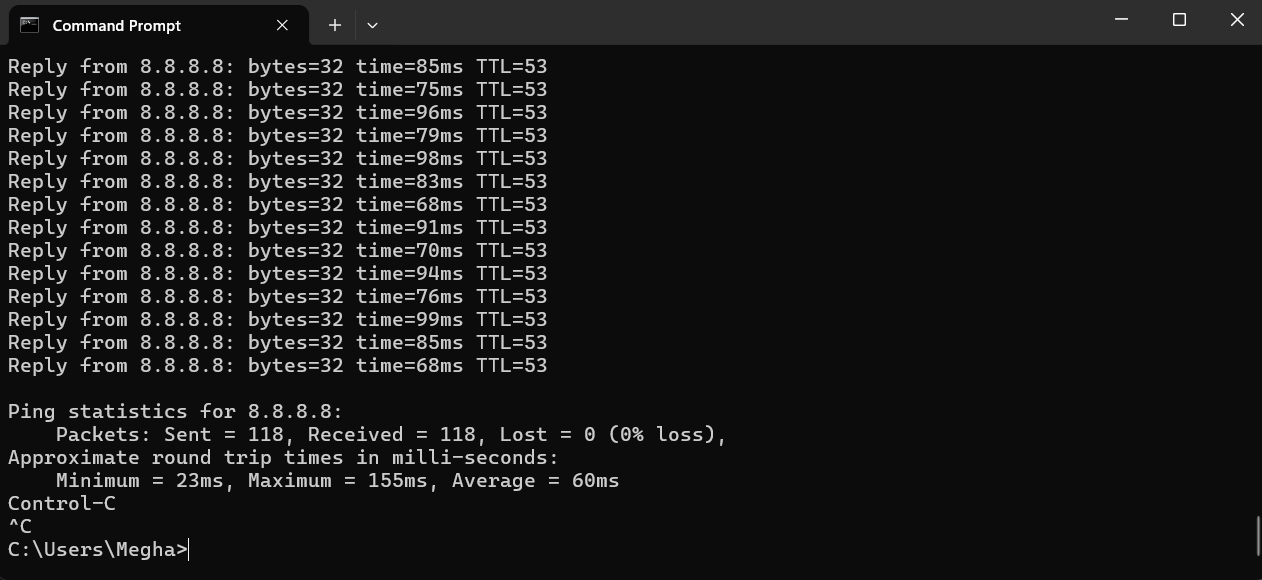
\includegraphics[width=0.8\linewidth]{Image/5g-streaming.png}
        \caption{Screenshot for 5G Network During Video Streaming}
        \label{fig:5g_streaming}
    \end{figure}

    \item \textbf{Video Calls:}
    \begin{itemize}
        \item \textbf{Time Started:} 431.5950s
        \item \textbf{Minimum Latency:} 24ms
        \item \textbf{Maximum Latency:} 88ms
        \item \textbf{Average Latency:} 42ms
        \item \textbf{Time Ended:} 552.1146s
    \end{itemize}
    \begin{figure}[h]
        \centering
        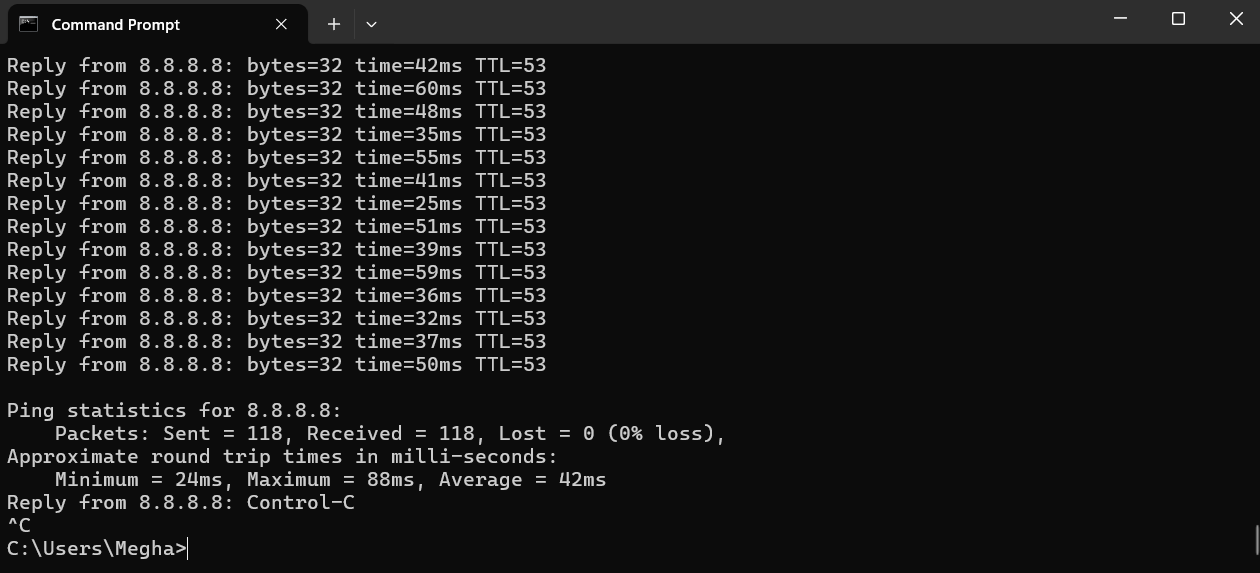
\includegraphics[width=0.8\linewidth]{Image/5g-video.png}
        \caption{Screenshot for 5G Network During Video Calls}
        \label{fig:5g_calls}
    \end{figure}

    \item \textbf{Gaming:}
    \begin{itemize}
        \item \textbf{Time Started:} 634.5442s
        \item \textbf{Minimum Latency:} 25ms
        \item \textbf{Maximum Latency:} 69ms
        \item \textbf{Average Latency:} 45ms
        \item \textbf{Time Ended:} 754.3583s
    \end{itemize}
    \begin{figure}[h]
        \centering
        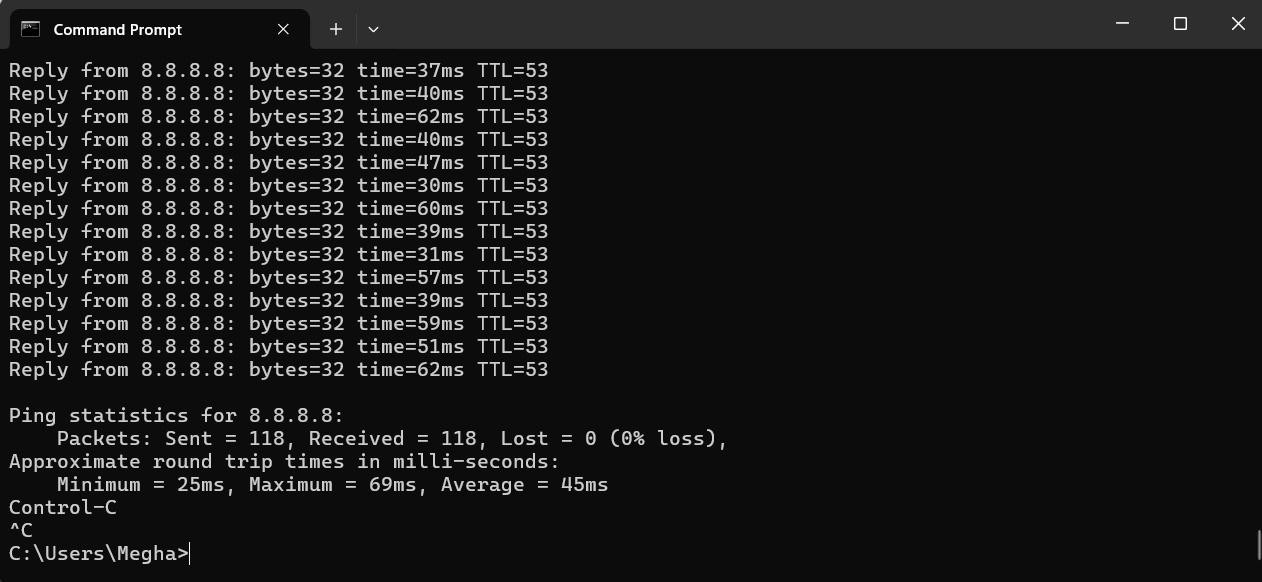
\includegraphics[width=0.8\linewidth]{Image/5g-gaming.png}
        \caption{Screenshot for 5G Network During Gaming}
        \label{fig:5g_gaming}
    \end{figure}

    \item \textbf{Downloading:}
    \begin{itemize}
        \item \textbf{Time Started:} 962.8064s
        \item \textbf{Minimum Latency:} 30ms
        \item \textbf{Maximum Latency:} 504ms
        \item \textbf{Average Latency:} 115ms
        \item \textbf{Time Ended:} 1084.888947s
    \end{itemize}
    \begin{figure}[h]
        \centering
        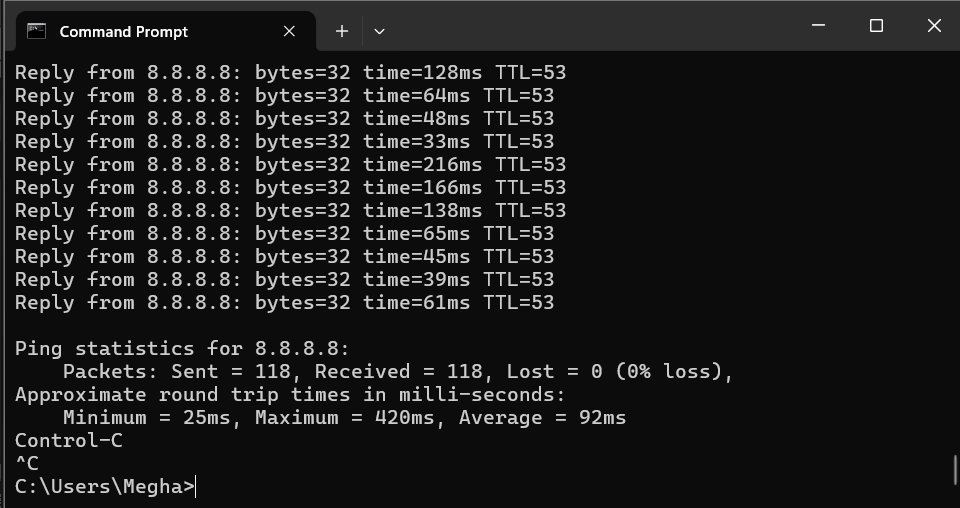
\includegraphics[width=0.8\linewidth]{Image/5g-download.png}
        \caption{Screenshot for 5G Network During Downloading}
        \label{fig:5g_downloading}
    \end{figure}
\end{itemize}

\subsection*{4G Network}
The following observations summarize the latency metrics for 4G under different scenarios.
\begin{itemize}
    \item \textbf{Idle (No Activity):}
    \begin{itemize}
        \item \textbf{Time Started:} 1211.635273s
        \item \textbf{Minimum Latency:} 35ms
        \item \textbf{Maximum Latency:} 78ms
        \item \textbf{Average Latency:} 46ms
        \item \textbf{Time Ended:} 1332.639354s
    \end{itemize}
    \begin{figure}[h]
        \centering
        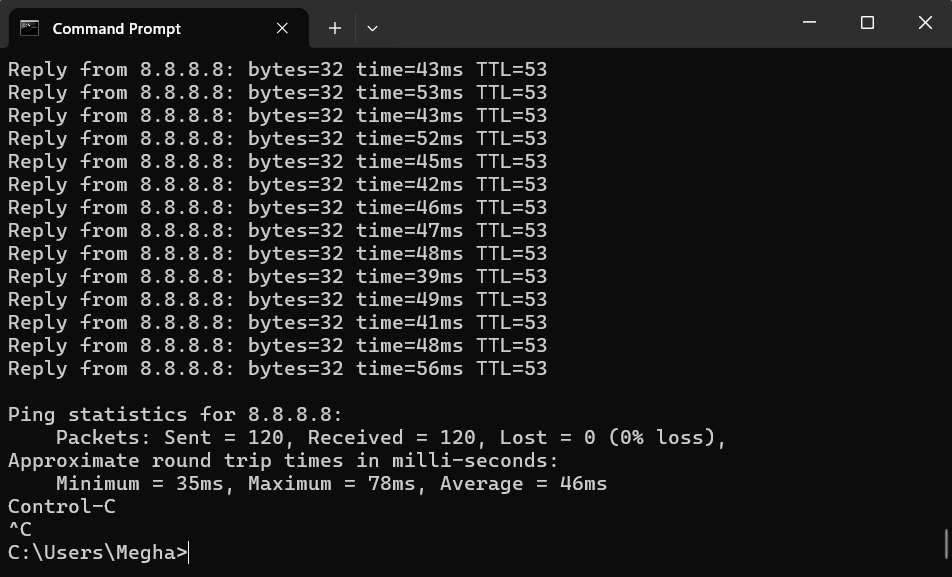
\includegraphics[width=0.8\linewidth]{Image/4g-idle.png}
        \caption{Screenshot for 4G Network Without Activity}
        \label{fig:4g_idle}
    \end{figure}

    \item \textbf{Video Streaming:}
    \begin{itemize}
        \item \textbf{Time Started:} 1400.162651s
        \item \textbf{Minimum Latency:} 34ms
        \item \textbf{Maximum Latency:} 590ms
        \item \textbf{Average Latency:} 68ms
        \item \textbf{Time Ended:} 1520.851601s
    \end{itemize}
    \begin{figure}[h]
        \centering
        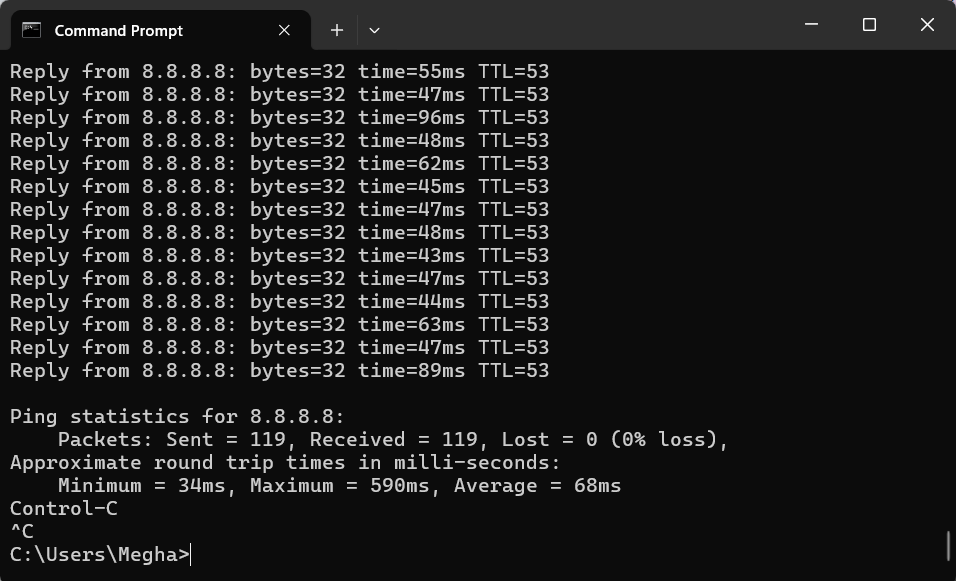
\includegraphics[width=0.8\linewidth]{Image/4g-streaming.png}
        \caption{Screenshot for 4G Network During Video Streaming}
        \label{fig:4g_streaming}
    \end{figure}
\newpage
    \item \textbf{Video Calls:}
    \begin{itemize}
        \item \textbf{Time Started:} 1650.245550s
        \item \textbf{Minimum Latency:} 33ms
        \item \textbf{Maximum Latency:} 113ms
        \item \textbf{Average Latency:} 44ms
        \item \textbf{Time Ended:} 1773.170535s
    \end{itemize}
    \begin{figure}[h]
        \centering
        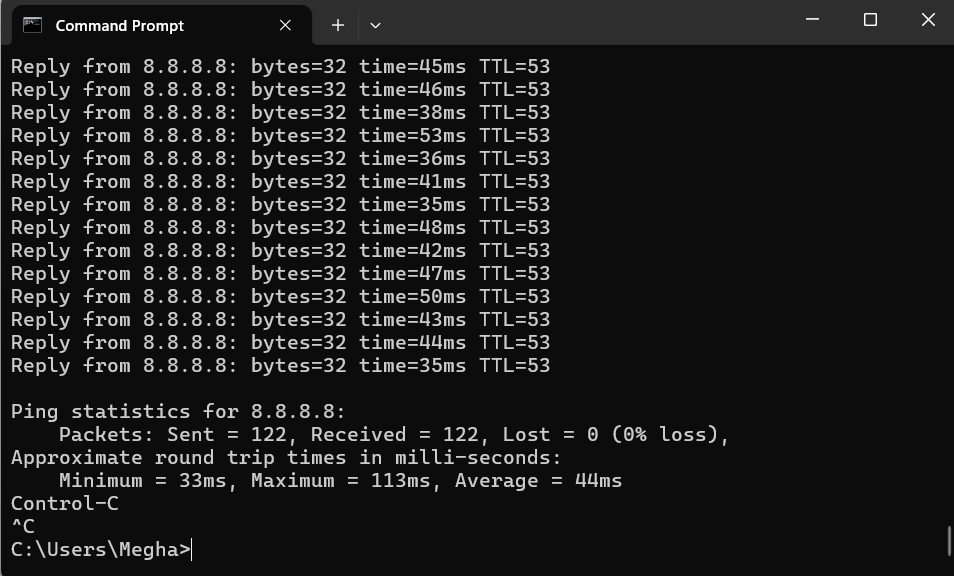
\includegraphics[width=0.8\linewidth]{Image/4g-video.png}
        \caption{Screenshot for 4G Network During Video Calls}
        \label{fig:4g_calls}
    \end{figure}

    \item \textbf{Gaming:}
    \begin{itemize}
        \item \textbf{Time Started:} 1995.226321s
        \item \textbf{Time Ended:} 2116.335060s
    \end{itemize}
    \begin{figure}[h]
        \centering
        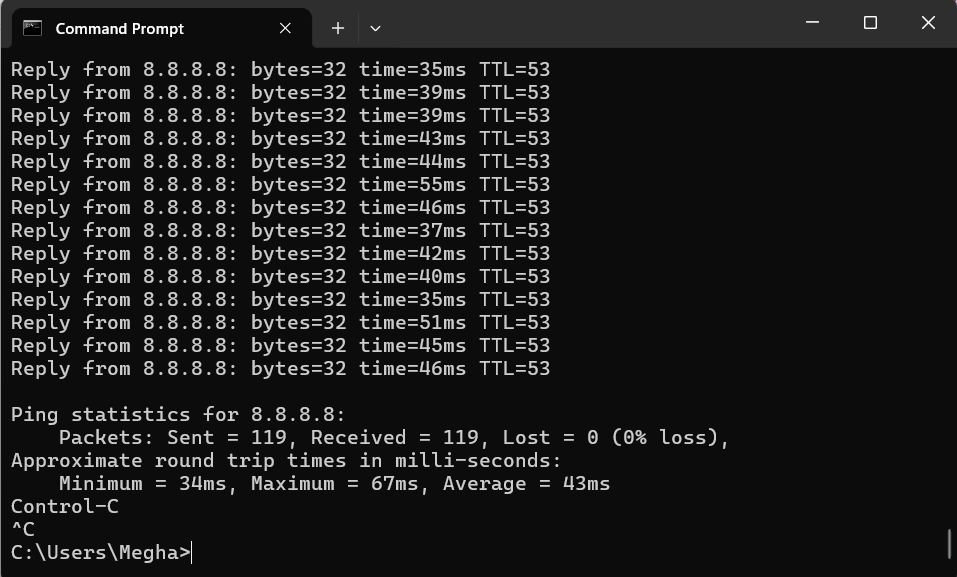
\includegraphics[width=0.8\linewidth]{Image/4g-gaming.png}
        \caption{Screenshot for 4G Network During Gaming}
        \label{fig:4g_gaming}
    \end{figure}

    \item \textbf{Downloading:}
    \begin{itemize}
        \item \textbf{Time Started:} 2325.101043s
        \item \textbf{Time Ended:} 2445.204007s
    \end{itemize}
    \begin{figure}[h]
        \centering
        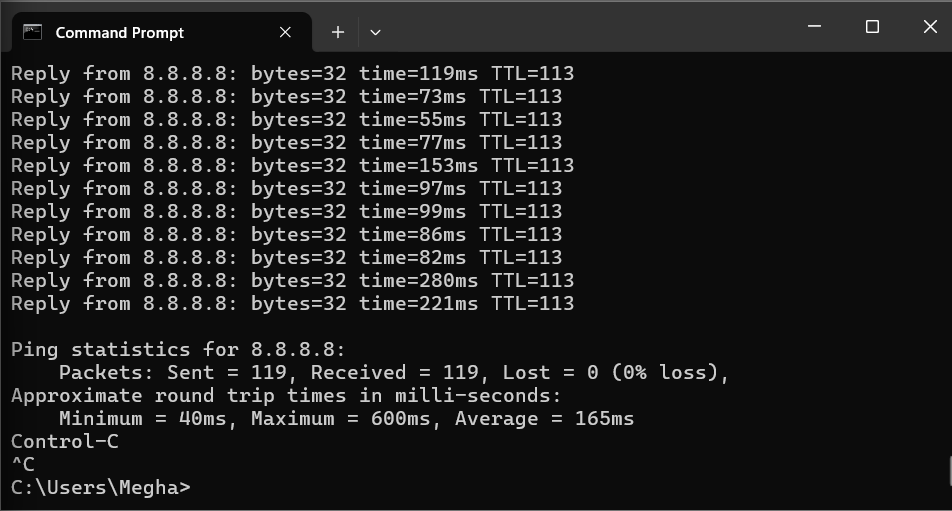
\includegraphics[width=0.8\linewidth]{Image/4g-download.png}
        \caption{Screenshot for 4G Network During Downloading}
        \label{fig:4g_downloading}
    \end{figure}
\end{itemize}




\section{Results}

\begin{itemize}
    \item \textbf{Idle Latency:}
    \begin{itemize}
        \item \textit{Minimum latency:} 5G achieved 27 ms, while 4G recorded 35 ms.
        \item \textit{Maximum latency:} 5G reached 80 ms, while 4G recorded 78 ms.
        \item \textit{Average latency:} 5G had 52 ms, while 4G recorded 46 ms.
    \end{itemize}
    
    \item \textbf{Video Streaming:}
    \begin{itemize}
        \item \textit{Minimum latency:} 5G achieved 23 ms, while 4G recorded 34 ms.
        \item \textit{Maximum latency:} 5G reached 155 ms, while 4G recorded 590 ms.
        \item \textit{Average latency:} 5G had 60 ms, while 4G recorded 68 ms.
    \end{itemize}
    
    \item \textbf{Video Calls:}
    \begin{itemize}
        \item \textit{Minimum latency:} 5G achieved 24 ms, while 4G recorded 33 ms.
        \item \textit{Maximum latency:} 5G reached 88 ms, while 4G recorded 113 ms.
        \item \textit{Average latency:} 5G had 42 ms, while 4G recorded 44 ms.
    \end{itemize}
    
    \item \textbf{Gaming:}
    \begin{itemize}
        \item \textit{Minimum latency:} 5G achieved 25 ms, while 4G recorded 34 ms.
        \item \textit{Maximum latency:} 5G reached 69 ms, while 4G recorded 67 ms.
        \item \textit{Average latency:} 5G had 45 ms, while 4G recorded 43 ms.
    \end{itemize}
    
    \item \textbf{Download:}
    \begin{itemize}
        \item \textit{Minimum latency:} 5G achieved 25 ms, while 4G recorded 40 ms.
        \item \textit{Maximum latency:} 5G reached 420 ms, while 4G recorded 600 ms.
        \item \textit{Average latency:} 5G had 92 ms, while 4G recorded 165 ms.
    \end{itemize}
\end{itemize}

\begin{figure}[h]
        \centering
        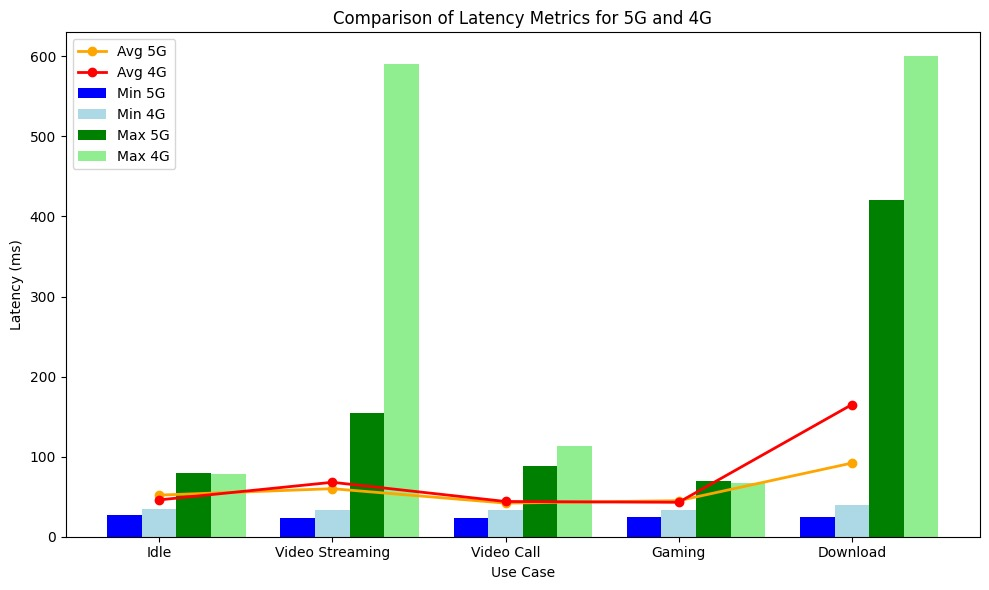
\includegraphics[width=0.8\linewidth]{Image/5G-project-graph.jpeg}
        \caption{Latency Comparison of 4G and 5G Across Use Cases}
        \label{fig:4g_gaming}
    \end{figure}

    \subsection{Graph Analysis}
The graph (Figure \ref{fig:4g_gaming}) provides a clear comparison of latency metrics for 5G and 4G across different use cases:

\begin{itemize}
    \item \textbf{5G Consistency:} 5G demonstrates lower average latency and smaller latency spikes in all use cases except idle, showcasing its reliability and suitability for applications like streaming, gaming, and video calls.
    \item \textbf{4G Latency Spikes:} The graph highlights significant maximum latency values for 4G, especially in video streaming and downloading tasks, which can impact user experience.
    \item \textbf{Use Case Performance:} For real-time and latency-sensitive applications like gaming and video calls, both networks perform comparably. However, 5G excels in scenarios requiring high bandwidth, such as downloads and streaming.
\end{itemize}

\section{Conclusion}

The results clearly demonstrate that 5G significantly outperforms 4G in most latency-related scenarios. Particularly for applications like video streaming and downloads, 5G exhibits lower minimum, maximum, and average latency, suggesting better reliability and responsiveness. However, in certain cases, such as idle and gaming, 5G’s average latency was slightly higher than 4G, indicating potential variability under specific conditions.

Overall, 5G's performance shows its potential for improving user experiences in latency-sensitive applications like video calls and streaming. However, variability in idle latency and gaming highlights the need for further optimization in real-world deployments. These findings reinforce the suitability of 5G for high-performance use cases but underline challenges that must be addressed for broader consistency.

\section{Contribution}
\begin{itemize}
    \item Megha Prajapati: 5G network analysis
    \item Vasireddy Satvika: 4G network analysis
    \item Sanya: Analyzed outputs and created graphs\newline
\end{itemize}

\textbf{Video link:} \href{https://drive.google.com/drive/folders/161ArB0oiu2vUooYZYLCOMglWWCVfffRn?usp=sharing }{Click here}

\end{document}
